\documentclass[UTF8,titlepage,twocolumn]{ctexart}
\CTEXsetup[format={\Large\bfseries}]{section}
\usepackage{amsmath}
\usepackage{caption}
\usepackage{graphicx}
\pagestyle{plain}
\title{弹性问题}
\date{\today}
\begin{document}
\maketitle

\section{模型}

令
$$
\begin{matrix}
	\sigma(u) = 2 \mu \epsilon(u) + \lambda tr(\epsilon(u)) \delta \\
	\epsilon(u) = \frac{1}{2} (grad u + (grad u)^t) \\
	tr(\tau) = \tau_{11} + \tau_{22} \\
	grad(u) = \begin{pmatrix}
		\frac{\partial u_1}{\partial x_1} & \frac{\partial u_1}{\partial x_2} \\
		\frac{\partial u_2}{\partial x_1} &
		\frac{\partial u_2}{\partial x_2}
	\end{pmatrix} \\
	\delta = \begin{pmatrix}
		1 & 0 \\
		0 & 1
	\end{pmatrix} \\
	div \tau = \begin{pmatrix}
		\frac{\partial \tau_{11}}{\partial x_1} + \frac{\partial \tau_{12}}{\partial x_2} \\
		\frac{\partial \tau_{12}}{\partial x_1} + \frac{\partial \tau_{22}}{\partial x_2}
	\end{pmatrix}
\end{matrix}
$$

考察模型
$$
\begin{matrix}
	-div \sigma(u) = f \quad \in \Omega  \\
	u |_{\Gamma} = 0
	%u |_{\Gamma_1} = g \\
	%(\sigma(u) \nu) |_{\Gamma2} = t
\end{matrix}
$$ 
\par
其中$ u = (u_1,u_2)^t $ 为求解向量,$ f = (f_1,f_2)^t $为右端向量,$ \Omega = [0,1] \times [0,1] $
$$
\begin{matrix}
	f_1 = -((12 x^2 - 12 x + 2) (4 y^3 - 6 y^2 
	\\ 
	+ 2 y) + (x - x^2)^2 (24 y - 12)) 
	\\
	f_2 = (24 x - 12)(y - y^2)^2 + (4 x^3 
	\\
	- 6 x^2 + 2 x) (12 y^2 - 12 y + 2)
\end{matrix}
$$

\section{变分}

该问题的变分问题为,求$u \in H^1(\Omega)$ 使得 $u |_{\Gamma_1} = g$,并且
$$
	a(u,\nu) = \int_{\Omega} f \cdot \nu dx \quad \forall \nu \in V
$$ 
\par
其中
$$
	\begin{matrix}
		a(u,\nu) := \int_{\Omega} (2 \mu \epsilon(u) : \epsilon(\nu) + \lambda div u div \nu) dx \\
		= \mu \int_{\Omega} \frac{\partial u_1}{\partial x} \frac{\partial \nu_1}{\partial x} + \frac{\partial u_1}{\partial y} \frac{\partial \nu_1}{\partial y} + \frac{\partial u_2}{\partial x} \frac{\partial \nu_2}{\partial x} + \frac{\partial u_2}{\partial y} \frac{\partial \nu_2}{\partial y} dx
		\\  
		+ (\mu + \lambda) \int_{\Omega} (\frac{\partial u_1}{\partial x} + \frac{\partial u_2}{\partial y}) (\frac{\partial \nu_1}{\partial x} \frac{\partial \nu_2}{\partial y}) dx
		\\
		V := \{ \nu \in H^1(\Omega) \quad | \quad \nu |_{\Gamma_1} = 0 \}
	\end{matrix}
$$

\section{三角形元}

\subsection{面积坐标}

设 $ \bigtriangleup(i,j,k) $ 是以 i,j,k 为定点的任意三角型元,面积为S。在 $ \bigtriangleup (p_0,p_1,p_2) $ 内任取一点$p_3$,坐标为(x,y)。过$p_3$点作与三个顶点的连线,将 $ \bigtriangleup(p_0,p_1,p_2) $ 分成三个三角形(图 1): $ \bigtriangleup(p_1,p_2,p_3), \bigtriangleup(p_0,p_3,p_2), \bigtriangleup(p_0,p_1,p_3) $,其面积分别为$S_0,S_1,S_2$

\begin{figure}[hb]
	\centering
	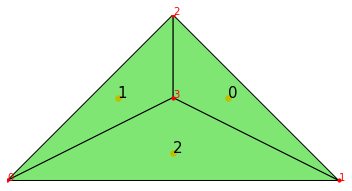
\includegraphics[height=3cm,width=4cm]{../image/TriangleElement.png}
	\caption{}
	\label{SampleOfDatasets}
\end{figure}

显然$S_0 + S_1 + S_2 = S$,令
$$
	L_0 = \frac{S_0}{S}, \quad L_1 = \frac{S_1}{S}, \quad L_2 = \frac{S_2}{S}
$$
\par
称$(L_0,L_1,L_2)$位$P_3$的面积坐标,其中
$$
	\begin{cases}
		2S = \left| \begin{matrix}
				1 & x_0 & y_0 \\
				1 & x_1 & y_1 \\
				1 & x_2 & y_2
			 \end{matrix} \right| ,
		 \quad
		 2S_0 = \left| \begin{matrix}
		 			1 & x   & y   \\
		 			1 & x_1 & y_1 \\
		 			1 & x_2 & y_2
		 \end{matrix} \right| 
		 \\
		2S_1 = \left| \begin{matrix}
					1 & x_0 & y_0 \\
					1 & x   & y   \\
					1 & x_2 & y_2
			   \end{matrix} \right|,
		\quad
		2S_2 = \left| \begin{matrix}
					1 & x_0 & y_0 \\
					1 & x_1 & y_1 \\
					1 & x   & y
			   \end{matrix} \right|
	\end{cases}
$$

由此可得面积坐标和直角坐标的转化关系
$$
\begin{cases}
	x = x_0 L_0 + x_1 L_1 + x_2 L_2 \\
	y = y_0 L_0 + y_1 L_1 + x_2 L_2
\end{cases}
$$
$$
	\begin{cases}
		L_0 = \frac{1}{2S} [(x_2 y_3 - x_3 y_2) + (y_2 - y_3) x + (x_3 - x_2) y] \\
		L_1 = \frac{1}{2S} [(x_3 y_0 - x_0 y_3) + (y_3 - y_0) x + (x_0 - x_3) y] \\
		L_2 = \frac{1}{2S} [(x_0 y_1 - x_1 y_0) + (y_0 - y_1) x + (x_1 - x_0) y]
	\end{cases} 
$$

\subsection{Lagrange型公式}

在三角型元$ \bigtriangleup(0,1,2) $上构造插值多项式
$$
	p_m(x,y) = \sum\limits_{i+j=0}^m c_{ij} x^i y^j
$$
\par
易知$p_m \in H^1$,当m=1时,有待定系数法得
$$
	p_1(x,y) = L_0 u_0 + L_1 u_1 + L_2 u_2
$$ 
\par
从公式可知$L_i$即为对应节点的基函数在单元$ \bigtriangleup(0,1,2) $上的限制。

\section{刚度矩阵}

\subsection{剖分}

对区间 $\Omega$ 按图2方式剖分,并对节点和区间进行编号,各节点坐标为$(x_i,y_i)$, i=0, ... , n

\begin{figure}[hb]
	\centering
	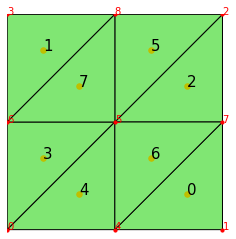
\includegraphics[height=4cm,width=4cm]{../image/subdivsion.png}
	\caption{}
\end{figure}

\subsection{总刚度矩阵}

设 $\phi_i = (\phi_i^{(1)}, \phi_i^{(2)})^t$,i = 0, ... , n 为试探函数空间$U_h$的基函数,则任一 $u_h \in U_h$ 可表成
$$
	u_h = \sum\limits_{i=1}^n u_i \phi_i, \quad u_i = u_h(x_i,y_i)
$$ 

带入变分形式得
$$
	\sum\limits_{j=0}^n a(\phi_j, \phi_i) u_i = (f,\phi_i) \quad i=0, ... ,n
$$

\subsection{单元刚度矩阵}

\end{document}